\section{Chamber Operation and Performance Monitoring}

\subsection{Choice of Gas}

The main requirements for the chamber gas were that it have reasonably low 
multiple scattering, allow for reasonable gas gains, have high drift velocities
in order to reduce the random background expected from M{\o}ller 
electrons and target-generated X-rays, and be inexpensive because of the 
large volume of the chambers. Also, safety considerations motivate the use of
a non-flammable gas mixture.  Additional concerns about small gas 
leaks and the proximity of many photomultiplier tubes argued against helium 
mixtures.  Ultimately a 90$\%$ argon - 10$\%$ CO$_2$ mixture was employed 
for several reasons: the gas has a fairly high saturated drift velocity 
($>$ 5~cm/$\mu$s), and it has an operating voltage plateau of several hundred 
volts before breakdown occurs.  The 90$\%$/10$\%$ mixture 
provides good efficiency and resolution, and reasonable collection times.

\subsection{Selecting the Proper Operating Voltage}

In this section we discuss our operating voltages and how they were determined.
First, we discuss how we divided the total voltage between our sense, field, 
and guard wires in order to mimic a cell layout with an infinite number of
layers, achieving a situation in which all wires, regardless of layer, have
the same gain.  Then we discuss our choice of the total sense to field
wire difference in voltage; including the resulting gas gain and efficiency.

\subsubsection{Dividing the Total Voltage between Sense, Field, and Guard Wires}

We ran our chambers with a mixed voltage scheme:
positive high voltage on the sense wires, negative voltage on the
field wires, and positive voltage on the guard wires.
This mixed-voltage scheme has several advantages over a scheme in
which the field wires, for example, are held at ground potential:
\begin{itemize}
\item fewer field lines run from the sense wire to the endplate, which
is grounded.  This reduces the likelihood of producing a ``Malter effect''~\cite{malter} in
which an accidental source of cathode emission
(due to an insulating contaminant on the endplate, for example) causes
a self-sustaining discharge;
\item the sense-to-ground potential and the field-to-ground potentials 
are smaller, decreasing surface electric fields on the on-chamber
circuit boards.
\end{itemize}

In addition, by selecting the values of the sense, field, and
guard wire voltages such that the net charge on all wires is zero, 
we create potential distributions that mimic
an infinite grid of cells, where the gain on any wire is the same as
any other, regardless of whether it is the first, last, or middle layer.

This optimum condition is reached when the sense voltage is twice the
field voltage (and opposite polarity).  This is because we have twice as many
field wires as sense wires and all field lines that originate on a
field wire land on a sense wire.  

The guard wire voltage was then chosen so that the total charge on all wires is zero.  
If we have a nearby ground plane due to the metallized gas window, in general
there will be an induced surface charge on the window 
that will affect the surface charge on the wires and
thus the gain of the nearby wire layers.  However, if the net charge on
all wires is zero, then there is no net flux of electric field through the
gas bag and thus the net charge on the gas bag is zero.  In this way all
of the wires have the same gain, regardless of layer.  
See Ref.~\cite{mdm92} for a discussion of these issues.

We used the drift chamber design program GARFIELD~\cite{GARFIELD} to determine the voltages
necessary to achieve the condition of net charge equal to zero.
The resulting ratio of voltages from sense to field to guard wires is 1 : -1/2 : 5/14.

\subsection{Determining the Operating Values of the Discriminator Thresholds and High Voltage Settings}
\label{determine-operating-parameters}

We set the discriminator levels in the DCRBs to reduce the accidental hit occupancy (with no beam) due to
electronic noise to be less than about 1\%.  Since the electronic noise was generally proportional to wire length,
we had less electronic noise on the smaller R1 chambers.  Using this criterion, we set the thresholds to 30, 45,
and 45~mV, respectively, for R1, R2, and R3.  
Once we set the discriminator thresholds, we performed a high voltage efficiency scan.  

We determined the layer efficiency using the ``excluded layer'' method.  In one superlayer (of six layers) we
found track segments by our usual fitting method, but ignoring the data from a pre-selected layer (layer 3, for
example).  We then projected the track segment through that layer and determined whether or not the indicated
wire (or an adjacent one) had a good hit.
We raised the sense to field wire potential in
steps of 75~V and analyzed the data.  We set the operating value for the high voltage at the point at which
the layer efficiency (the probability that a track passing through a layer will fire at least one wire) equaled or
exceeded 97\%.

% Fig.~\ref{effcy-vs-voltage} shows the ``plateau curve'' of efficiency
%plotted versus voltage for one typical chamber and superlayer.  The layer efficiency at the chosen operating high
%voltage point was between 97\% and 98\%.

%%%%%%%%%%%%%%%%%%%%%%%%%%%%%%%%%%%%%%%%%%%%%%%%%%%%%%%%%%%%%%%%%
%\begin{figure}[htbp]a
%\vspace{5cm}
%\begin{picture}(50,50)
%\put(-10,10)
%{\hbox{\includegraphics[width=0.35\textwidth,natwidth=610,natheight=642]{img/trace-routing-schematic.jpg}}}
%\end{picture}
%\caption{\small{Layer efficiency plotted versus high voltage for a typical superlayer.}}
%\label{effcy-vs-voltage}
%\end{figure}
%%%%%%%%%%%%%%%%%%%%%%%%%%%%%%%%%%%%%%%%%%%%%%%%%%%%%%%%%%%%%%%%%

\subsubsection{Operating Voltage and Gas Gain}
\label{operating-voltage}

The gas gain varies exponentially with the total sense to field wire voltage
difference, with a doubling voltage of about 100, 110, or 120~V, respectively, for
R1, R2, and R3.  During our fall 2018 run, we ran with sense - field wire voltage
differences of 2100, 2325, and 2475~V, respectively, for R1, R2, and R3.
We calculate that our total gas gain is approximately 
$2.7 \times 10^4$, $3.7 \times 10^4$, and $4.4 \times 10^4$,  
respectively, for R1, R2, and R3.

\subsection{In-Run Performance Monitoring}

The CLAS12 detector records 10,000 - 20,000~events/s during a typical experiment.
It is important that the experimenters who are running the data-taking be quickly
aware of any equipment malfunctions.

Our first level of monitoring comes from our hardware alarms; see Section~\ref{utilities}
to see images of the control panels for our gas system and power
supplies.  Should these malfunction, an alarm is instantly shown on an alarm summary
screen with GUI-driven information on the lower-lying hardware monitoring screens.
An experimenter is thus able to detect an alarm, and in most cases, reset the
alarming supply, within minutes.

Our second level of monitoring comes from on-line accumulating histograms.
Of these, the most important are our so-called ``Occupancy Plots'', which
are simply histograms of wire hits plotted versus wire number and wire layer (summed over
six superlayers in each sector).  Malfunctions show up
as depleted areas on the plots.

Figure~\ref{layer-vs-wire} shows a histogram of wire hits plotted as
a function of layer (1 - 36 on the vertical scale) versus wire number for each of the six
sectors.  A R1 chamber contains layers 1 - 12, a R2 chamber layers 13 - 24, and a 
R3 chamber layers 25 - 36. The horizontal axis shows the wire number in each layer (1 - 112).  
At a glance, one can inspect our 24,000 wires and determine
that $>99\%$ of wires are functioning properly.  A few areas of inefficiency
are visible in the upper middle graph, corresponding to
two areas in which the HV was disconnected to stop excessive current draw.

%%%%%%%%%%%%%%%%%%%%%%%%%%%%%%%%%%%%%%%%%%%%%%%%%%%%%%%%%%%%%%
\begin{figure}[hbtp]
\vspace{7cm}
\begin{picture}(50,50)
\put(70,-5)
{\hbox{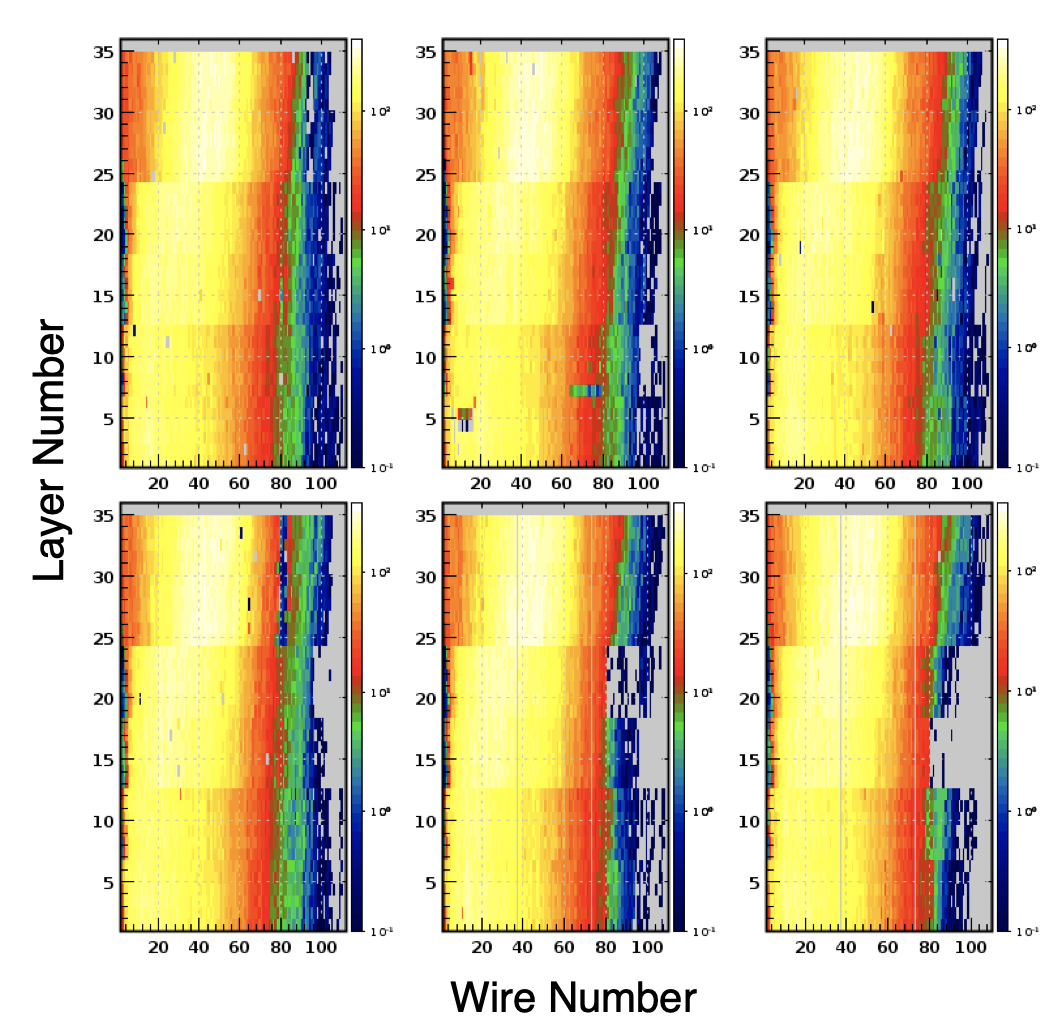
\includegraphics[width=0.75\textwidth,natwidth=610,natheight=642]{img/layer-vs-wire.png}}}
\end{picture}
\caption{\small{An ``occupancy plot'' showing the number of wire hits accumulated over many events.
A few malfunctioning wire groups can be seen in the upper middle graph.}}
\label{layer-vs-wire}
\end{figure}
%%%%%%%%%%%%%%%%%%%%%%%%%%%%%%%%%%%%%%%%%%%%%%%%%%%%%%%%%%%%%%
